%% Requires compilation with XeLaTeX or LuaLaTeX
%% based on UC Berkeley Beamer theme https://www.overleaf.com/latex/templates/uc-berkeley-beamer-theme/bywswngntrws
\documentclass[10pt,xcolor={table,dvipsnames},t]{beamer}

\usetheme{UCBerkeley}
\setbeamertemplate{footline}[frame number] 
\RequirePackage[style=numeric]{biblatex}
\addbibresource{refs.bib}
\RequirePackage{csquotes}
\RequirePackage{amsmath}
\RequirePackage{physics}
\RequirePackage{graphicx}
\RequirePackage[font=small]{caption, subcaption}
\RequirePackage{wrapfig}
\RequirePackage{siunitx}
\RequirePackage{sidecap}
\RequirePackage{caption}
\RequirePackage{booktabs}
\captionsetup[figure]{font = scriptsize, labelfont = scriptsize} % https://tex.stackexchange.com/questions/52132/beamer-change-size-of-figure-caption
\setkeys{Gin}{width=1\linewidth}


\title[Autosailboat]{Autonomous control of a sailboat}
\author{Neelay Junnarkar, Andrew Fearing, Hamza Khawaja}
% \institute{Your Faculty/Department}
\date{\today}

\begin{document}

\begin{frame}
  \titlepage
\end{frame}

\begin{frame}{Outline}
 \tableofcontents
\end{frame}
\section{Introduction}
\begin{frame}{Team}

Neelay Junnarkar

\hfill\\
Andrew Fearing

\hfill\\
Hamza Khawaja
\end{frame}


\begin{frame}{Motivation}
\begin{columns}
\column{0.5\linewidth}
    \begin{figure}
        \centering
        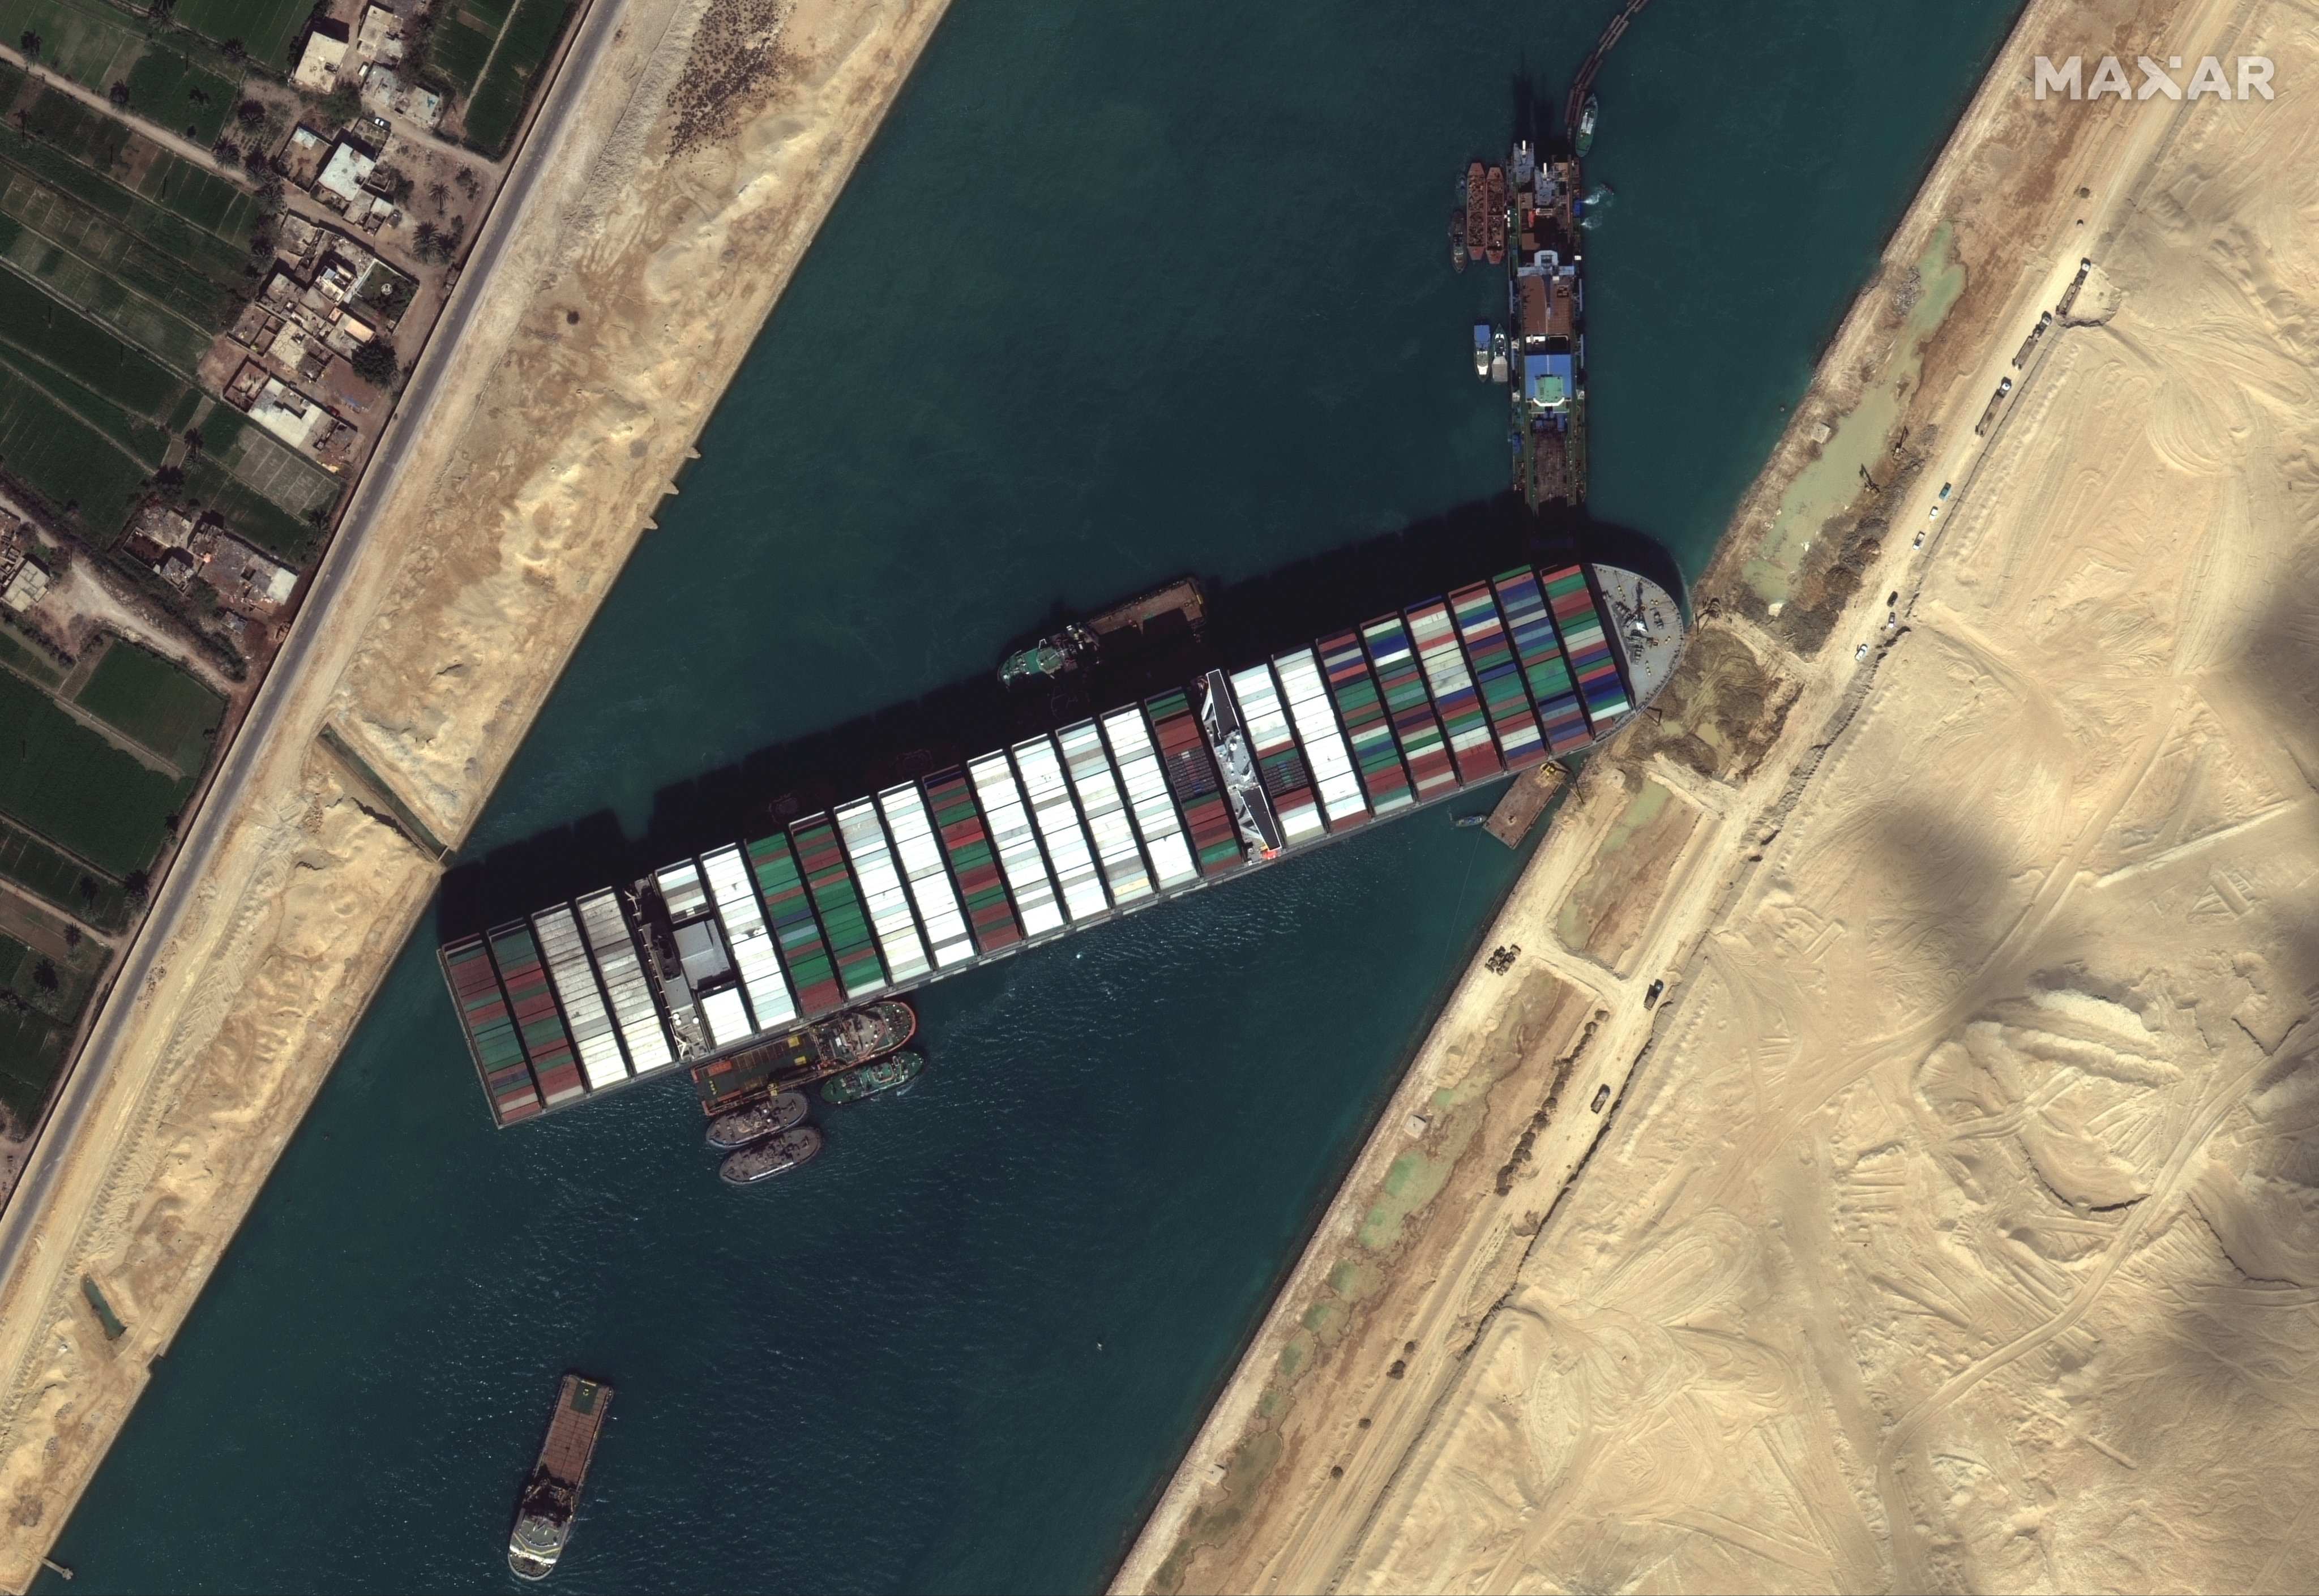
\includegraphics{documents/figures/Suez_Canal_blocked_by_Ever_Given_March_27_2021.jpg}
        \caption{Boat stuck}
        \label{fig:boat_stuck}
    \end{figure}  
\column{0.5\linewidth}
    \textbf{Control of sailboats}
    
    \hfill\\
    Controlling boats autonomously presents an interesting challenge due to the large effect of environmental disturbances such as wind, water currents, and waves. 
    
    \hfill\\
    \textbf{Why Sailboats?}
    
    \hfill\\
    Sailboats are useful for low-power long-term deployments. Also, present a gap in current literature,
    especially in controller design.
    
\end{columns}
\end{frame}

\begin{frame}{Goal}

\begin{enumerate}
    \item Develop sailboat yaw controller.
    \item Develop path planner which can navigate channels.
\end{enumerate}
Focus on robustness to environmental disturbances.

\end{frame}
  

\begin{frame}{Sailing}
\begin{columns}
\column{0.5\linewidth}

\begin{figure}
    \centering
    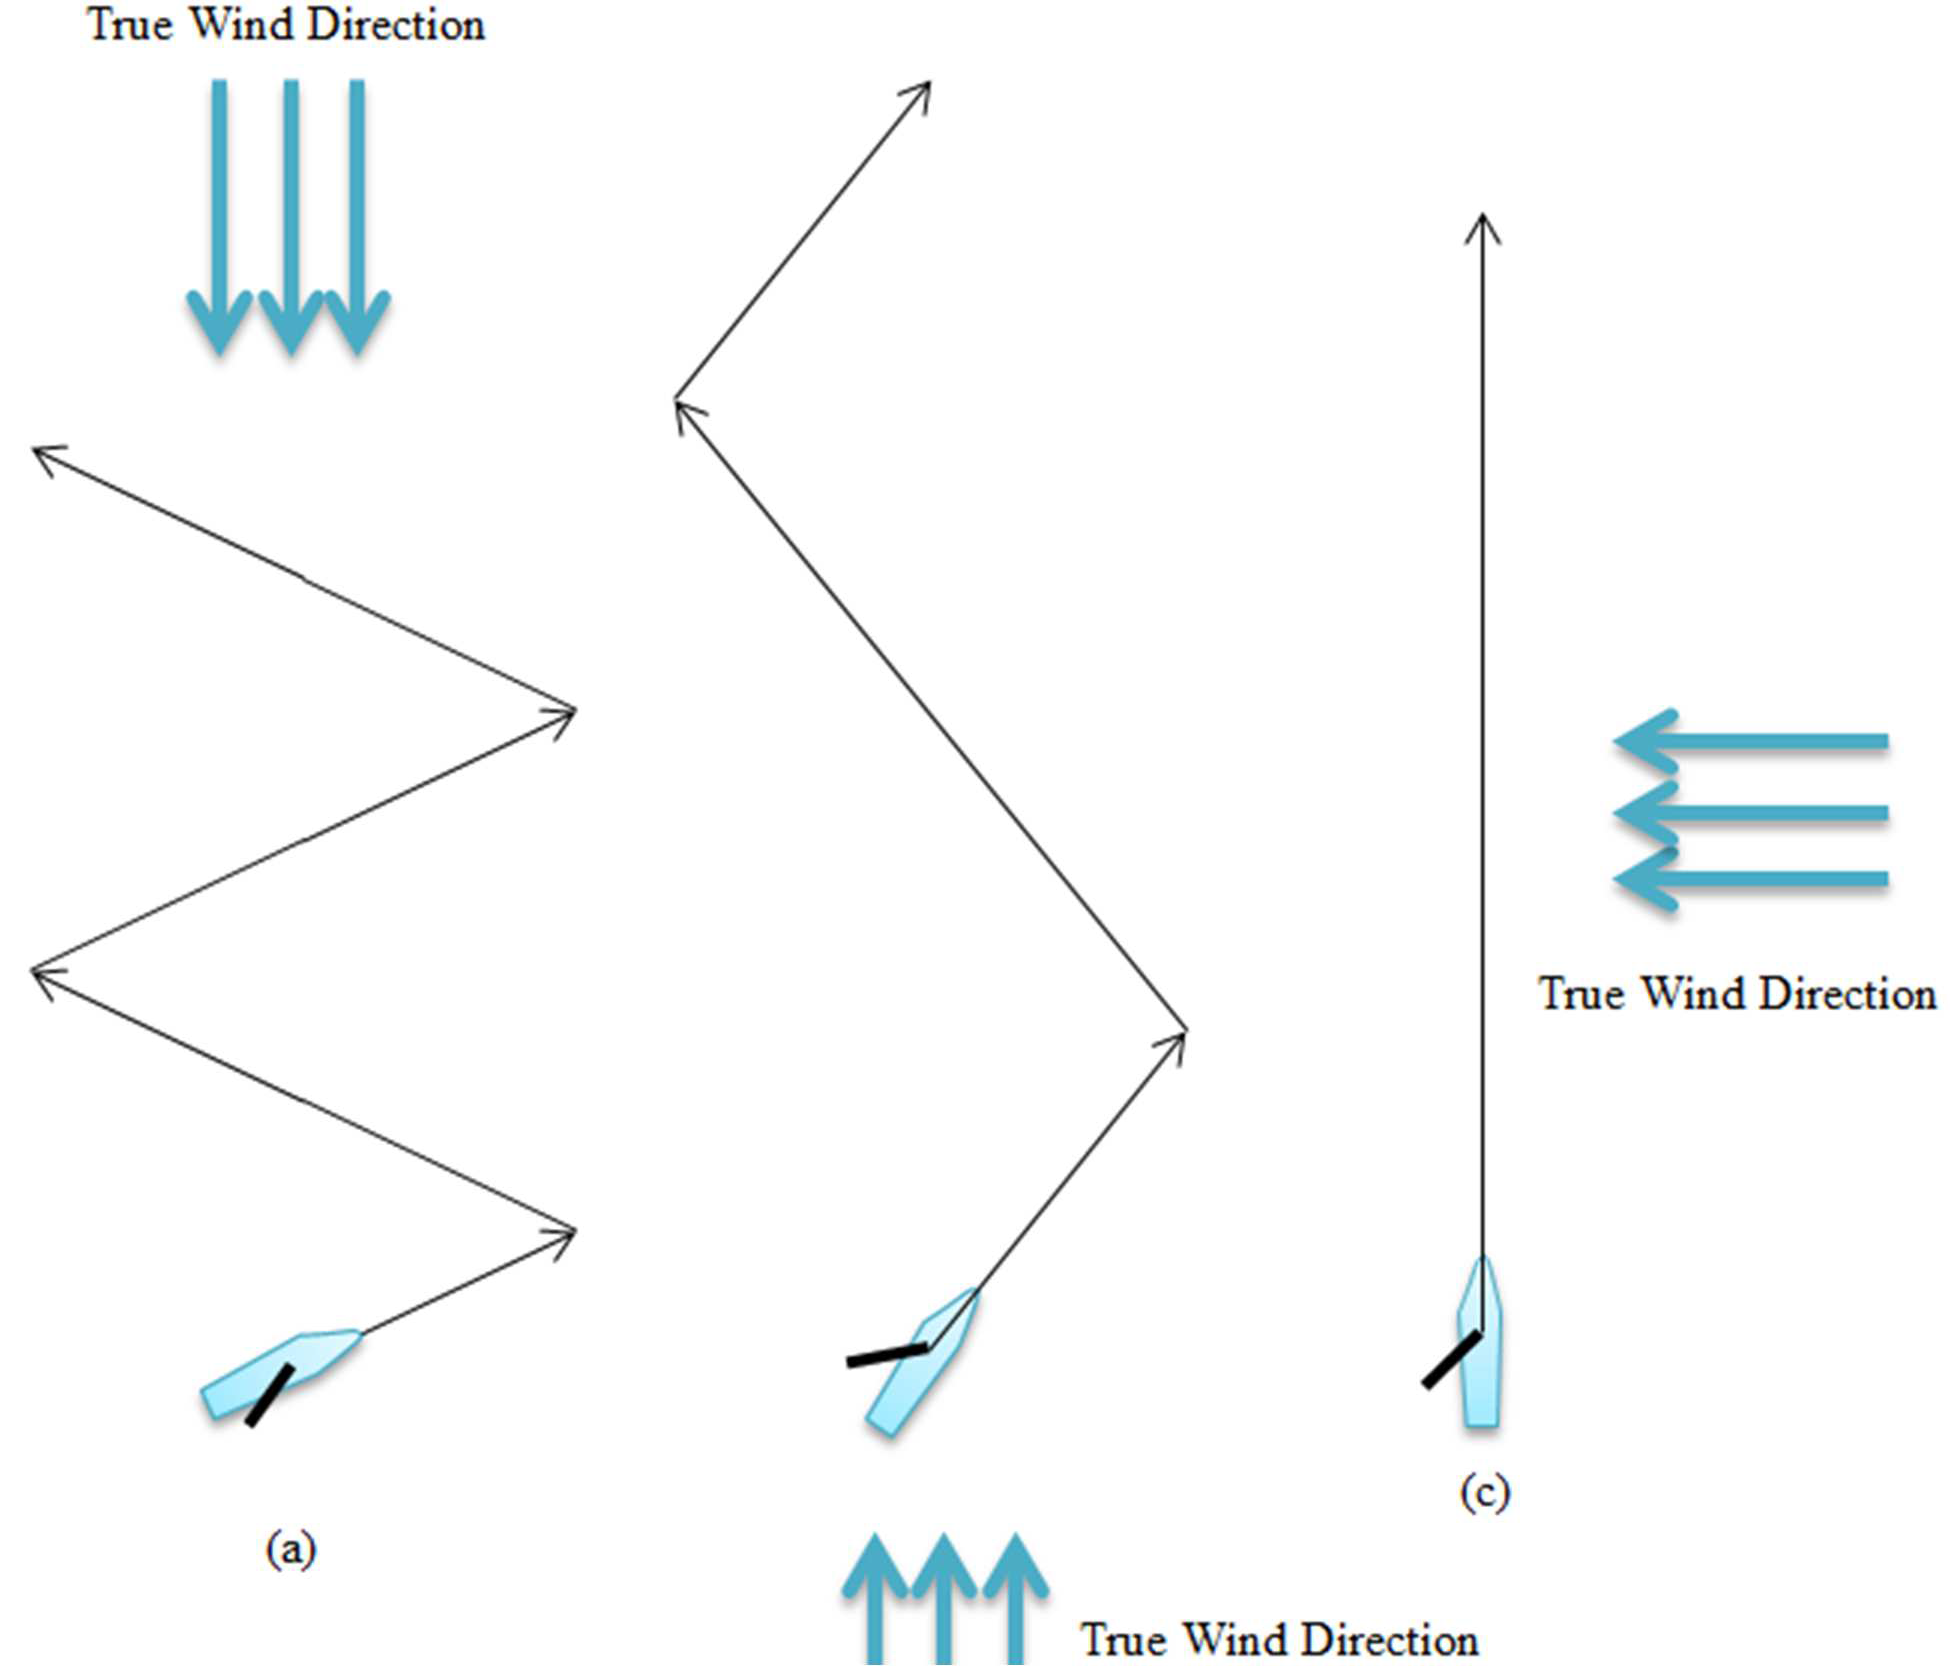
\includegraphics[width=\linewidth]{documents/figures/alves_modes.png}
    \caption{Modes of sailing \cite{Alves2010}}
    \label{fig:alves_modes}
\end{figure}
\column{0.5\linewidth}
\begin{figure}
    \centering
    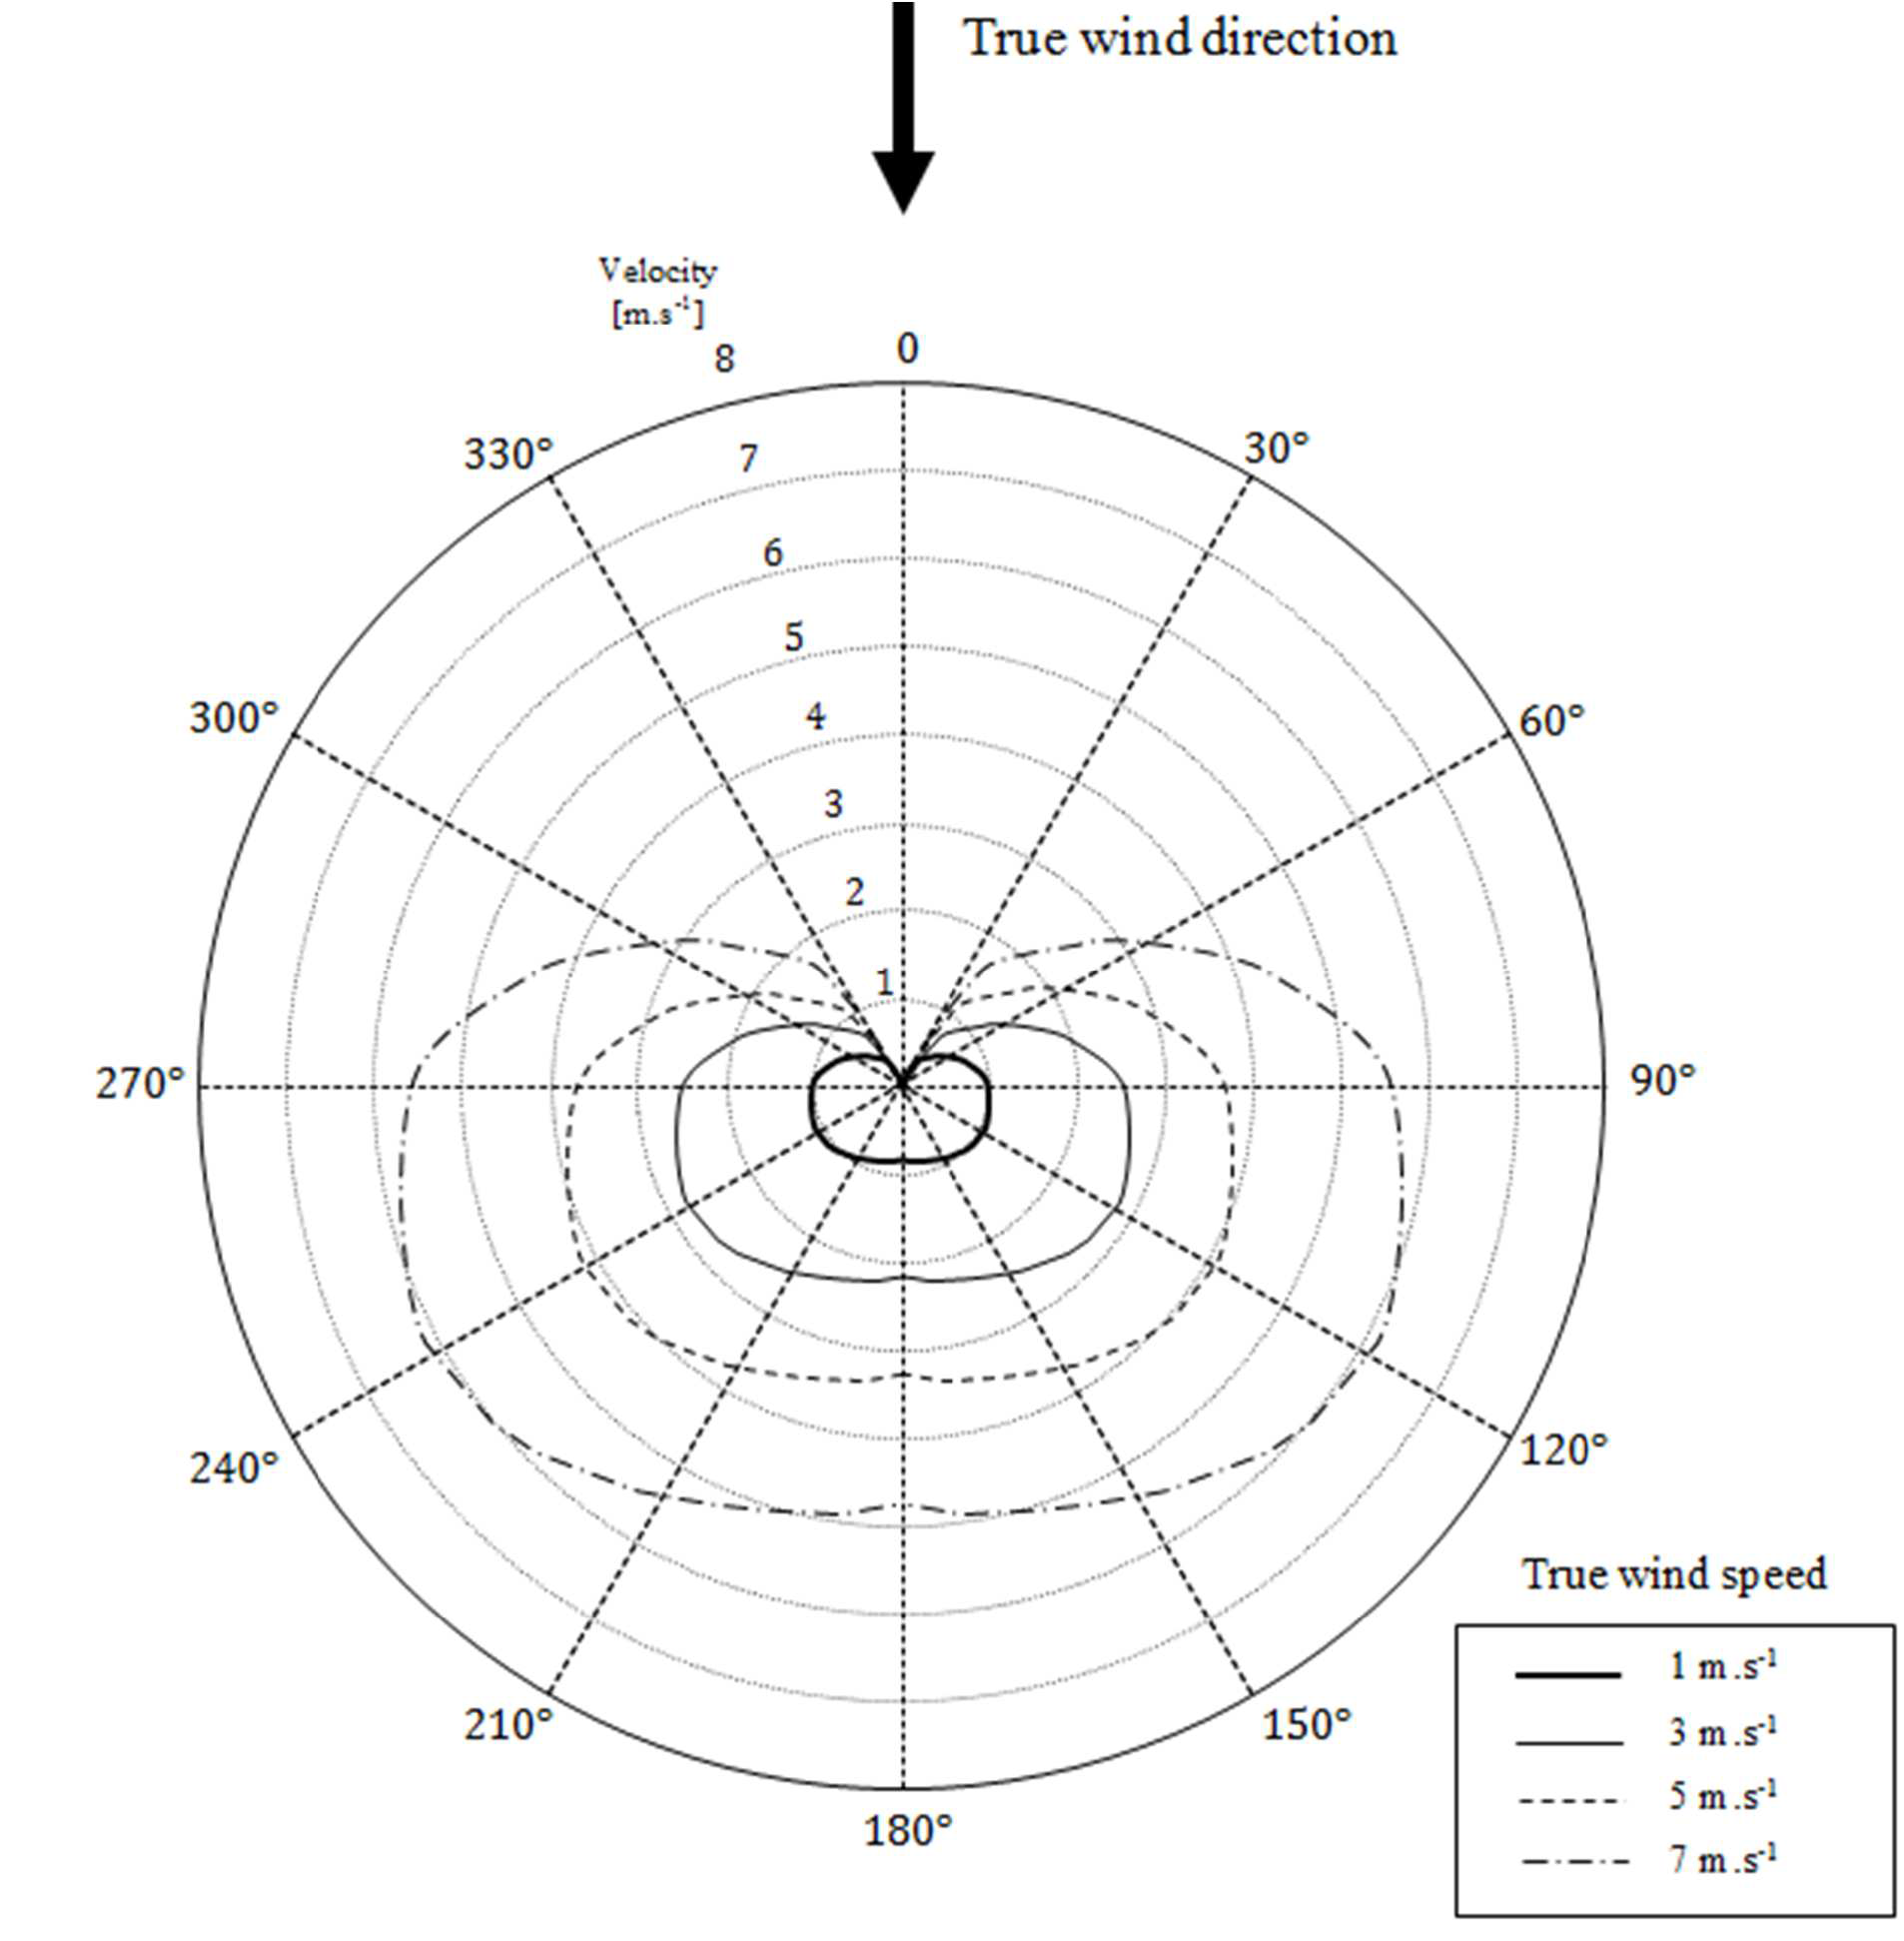
\includegraphics[width=\linewidth]{documents/figures/alves_vpp.png}
    \caption{Velocity polar diagram \cite{Alves2010}}
    \label{fig:alves_velocity}
\end{figure}
\end{columns}
\centerline{Sailboats trajectories depend on wind direction}
\end{frame}

\subsection{Sailboat model}

\begin{frame}{Sailboat Components}
\begin{columns}
\column{0.5\linewidth}
    \begin{figure}
        \centering
        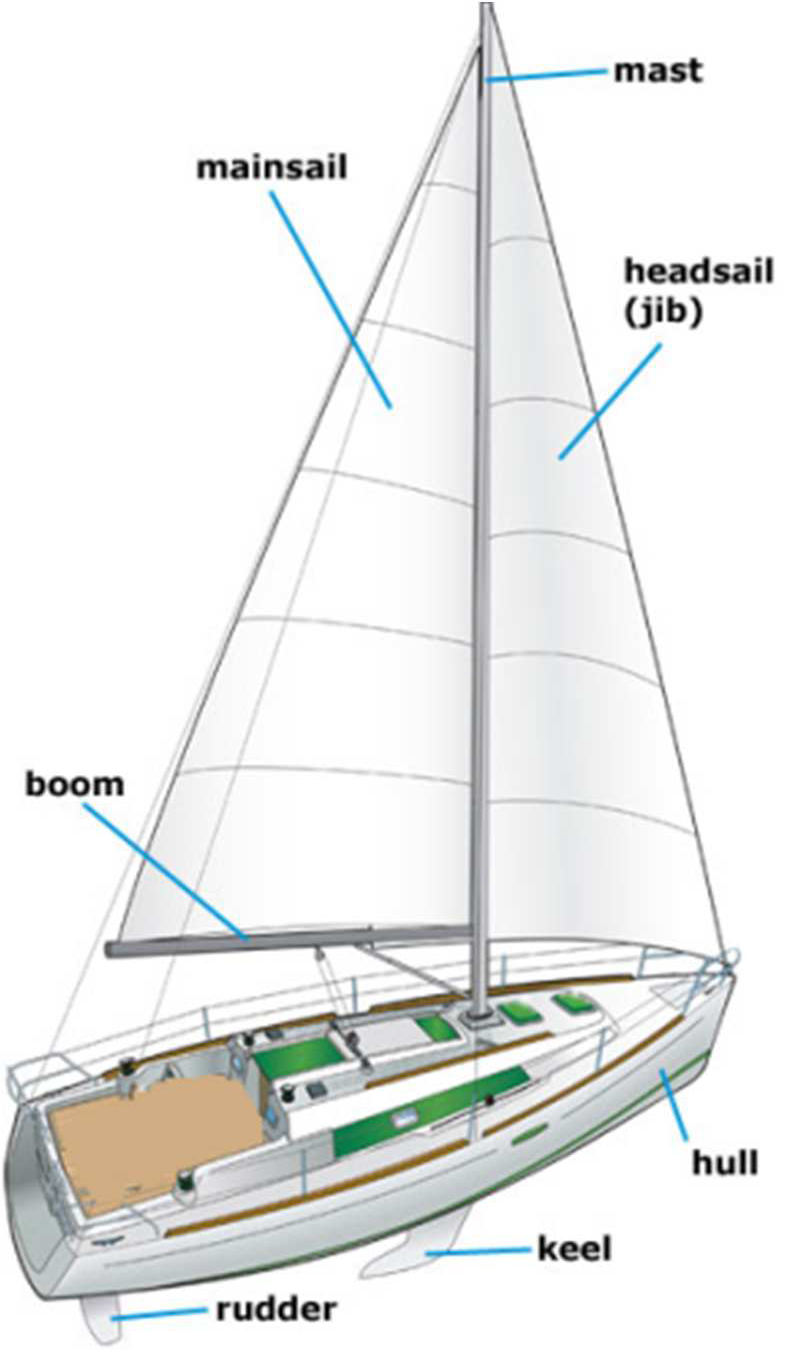
\includegraphics[height = 0.6\textheight, keepaspectratio]{documents/figures/alves_sailboat.png}
        \caption{Sailboat main components~\cite{Alves2010}.}
        \label{fig:my_label}
    \end{figure}
\column{0.5\linewidth}
\begin{itemize}
    \item Note that headsail and mainsail are connected in our model for simplicity
    \item Two control surfaces: sail and rudder \(\implies\) two actuators
\end{itemize}
\end{columns}

\end{frame}

\begin{frame}{6-DoF Model Axes}
\begin{table}[h]
    \centering
    \begin{tabular}{cc}
         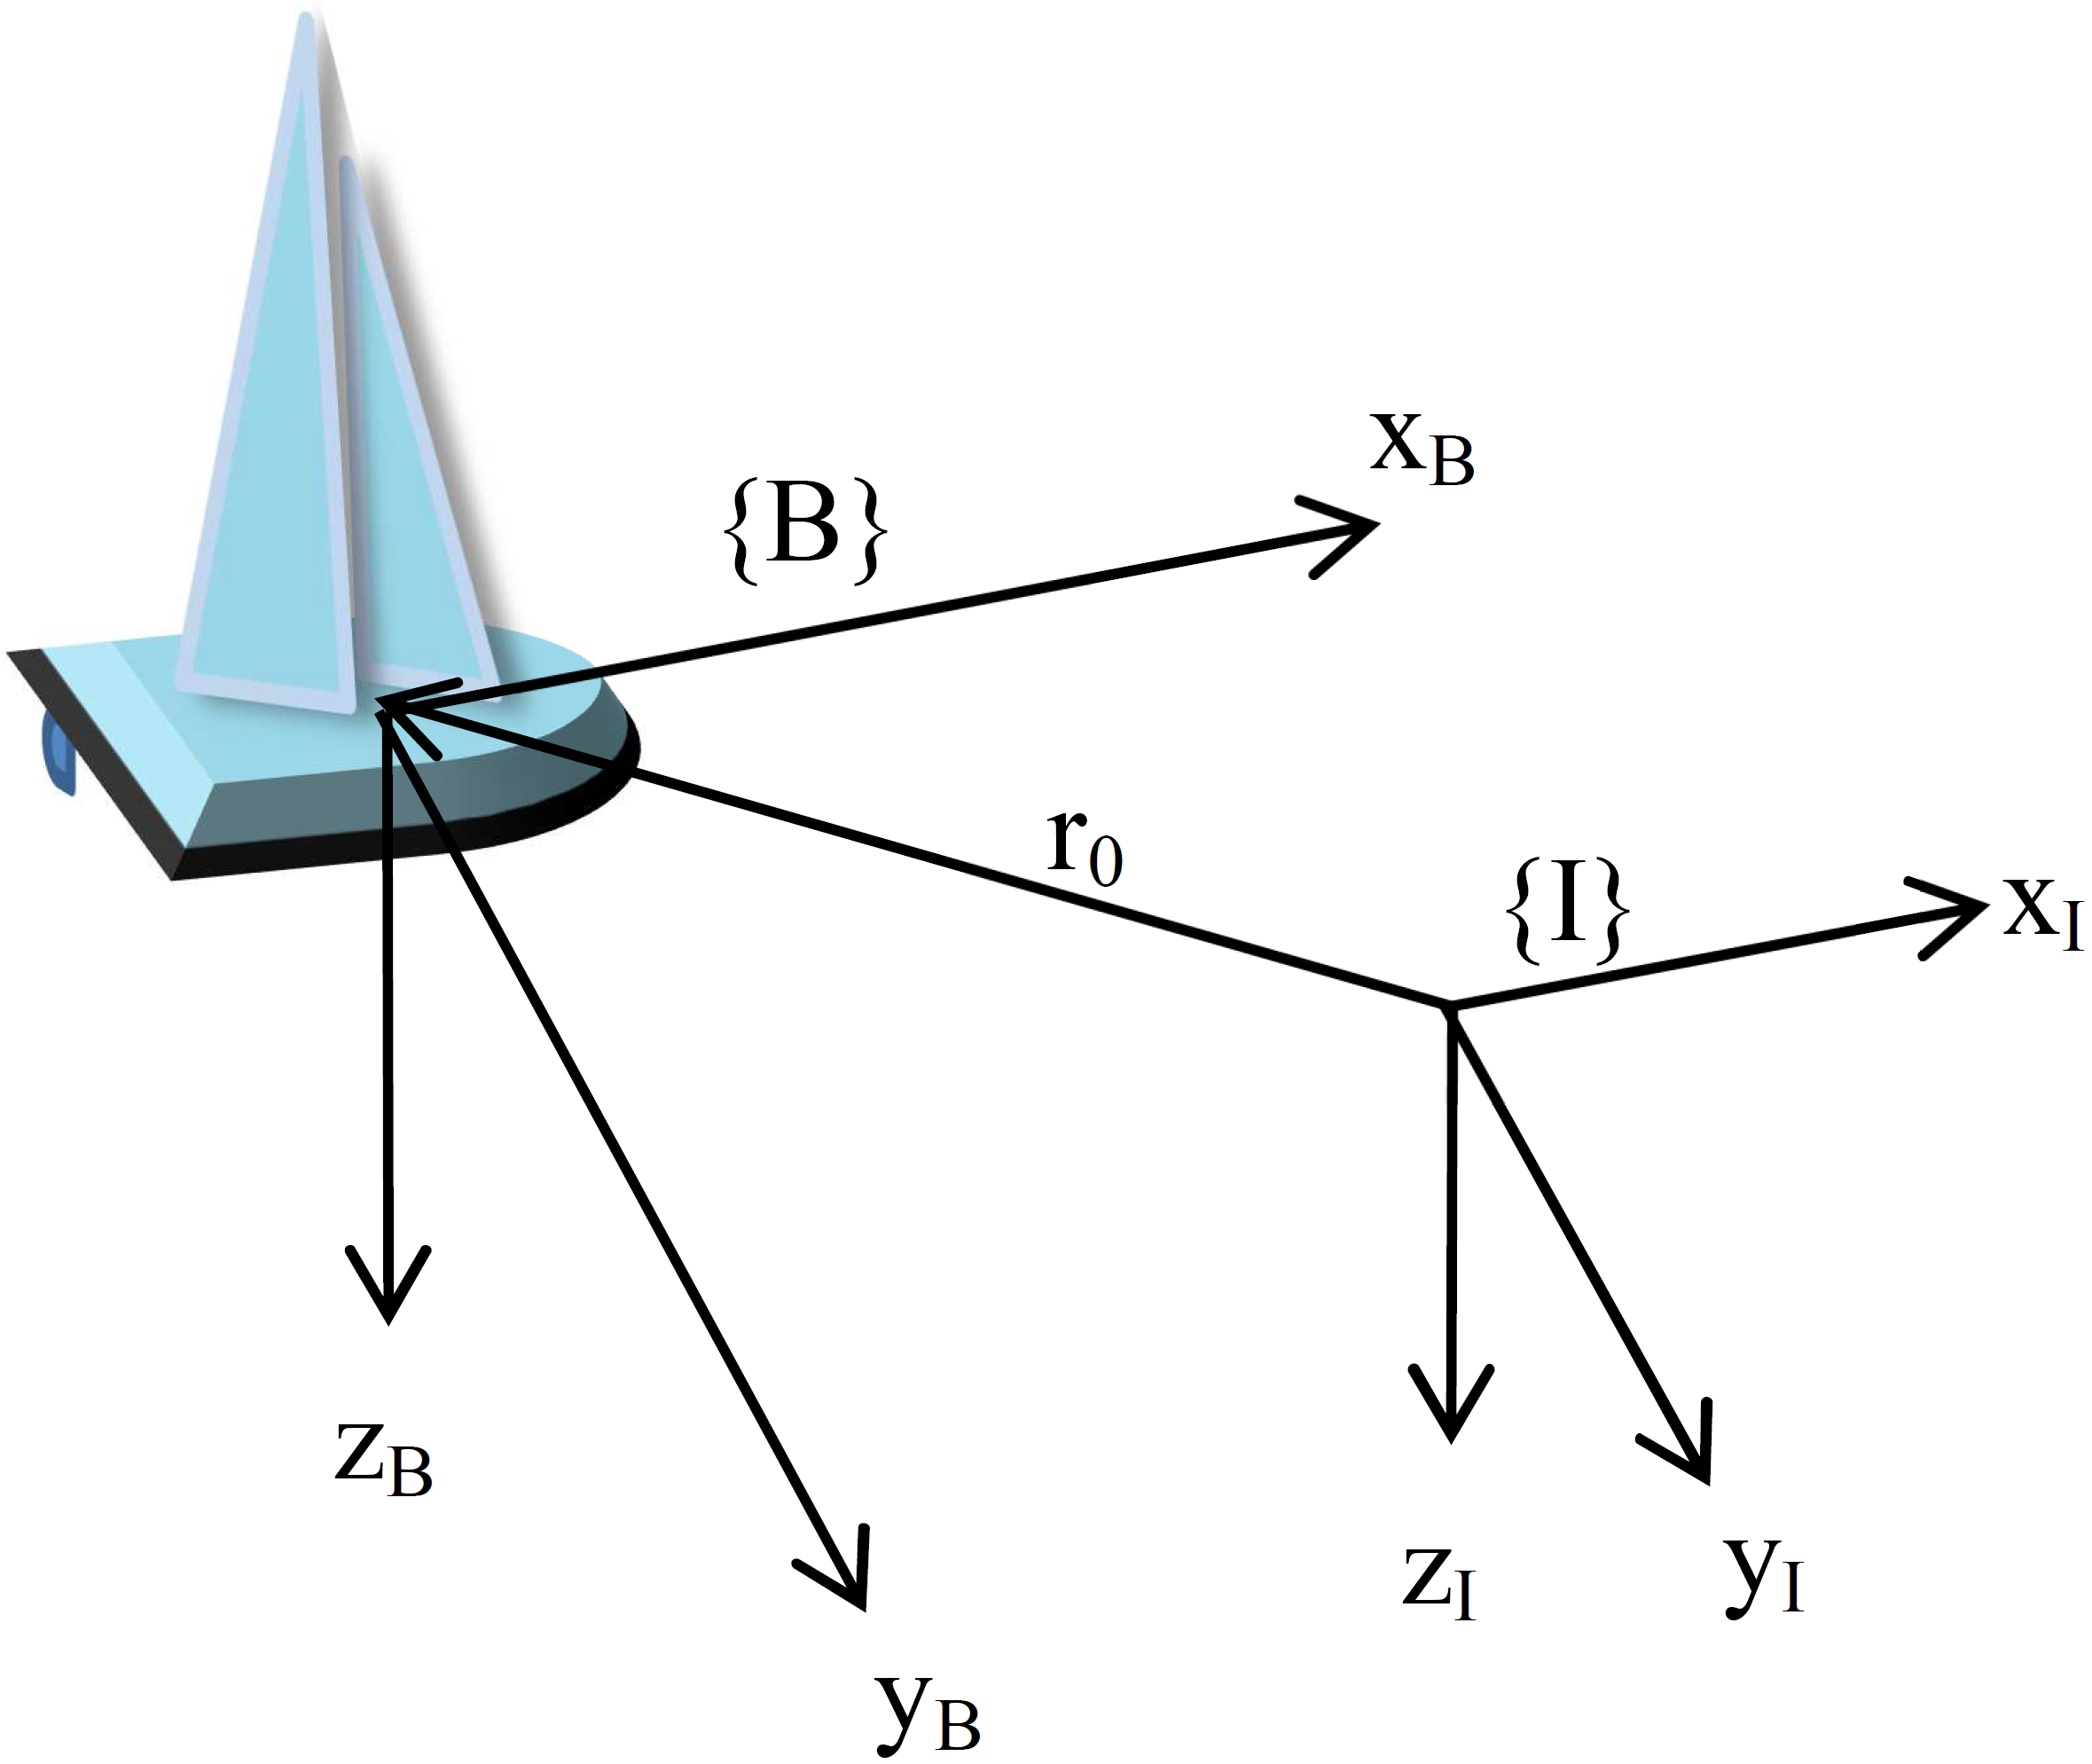
\includegraphics[width = 0.35\linewidth]{documents/figures/alves_frames.png} & 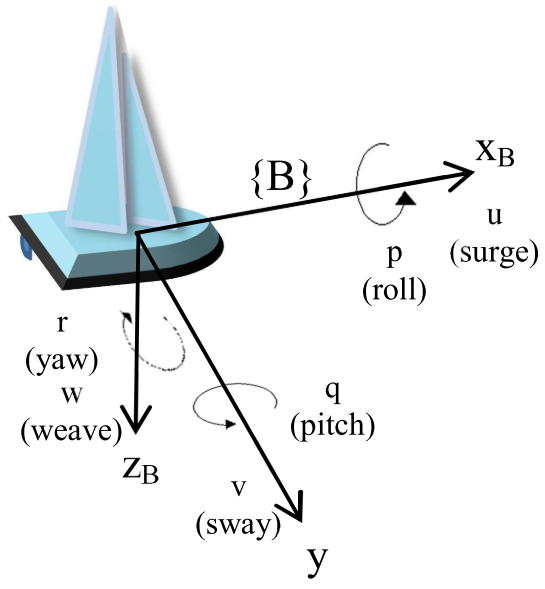
\includegraphics[width = 0.35\linewidth]{documents/figures/alves_rpy.png} \\
         Translation axes x-y-z           & Rotation axes roll-pitch-yaw \\
    \end{tabular}
    \caption{Axes}
    \label{tab:fig_axes}
\end{table}
    
\end{frame}




\section{Simulator}
\begin{frame}{Evaluating Simulators}
    
    
    Simulators for sailboat models are significantly underdeveloped.
    
    \begin{columns}
    \column{0.5\linewidth}
        \centerline{\texttt{USVSim} \cite{Paravisi2019}}
        \begin{itemize}
            \item Ubuntu 16.04 + Kinetic ROS + Gazebo
            \item 6 DoF boat dynamics model.
            \item Waves, buoyancy, water currents, wind currents, thruster underwater, thruster above water, foil
            \item Too complicated to work with, hard to extend
        \end{itemize}
    \column{0.5\linewidth}
        \centerline{\texttt{stda-sailboat-sim} \cite{Buehler2018}}
        \begin{itemize}
            \item Python + Numpy + Matplotlib
            \item 6 DoF boat dynamics model.
            \item Waves, buoyancy, wind, sail, keel, rudder forces.
            \item Good enough 
        \end{itemize}
    \end{columns}
    
\end{frame}



\begin{frame}{Rewriting Simulator}

    \texttt{stda-sailboat-sim} simulator appears to have been written just enough to satisfy the needs of the authors paper.
    
    \hfill\\
    We rewrote it significantly to modularize the code and allow easy and structured definition
    of controllers and path planners.

\end{frame}

% \begin{frame}{Simulation Results}
% \begin{table}[h]
%     \centering
%     \begin{tabular}{lcc}
%     x-y trajectory & 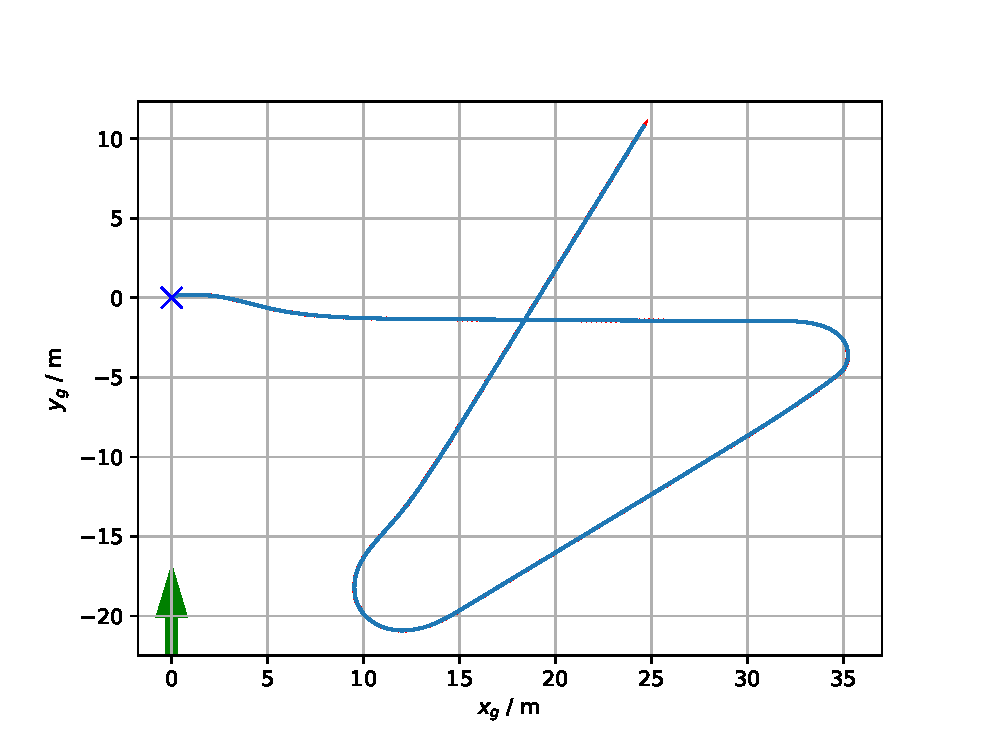
\includegraphics[width = 0.35\linewidth]{documents/figures/trajectories.eps} &
%     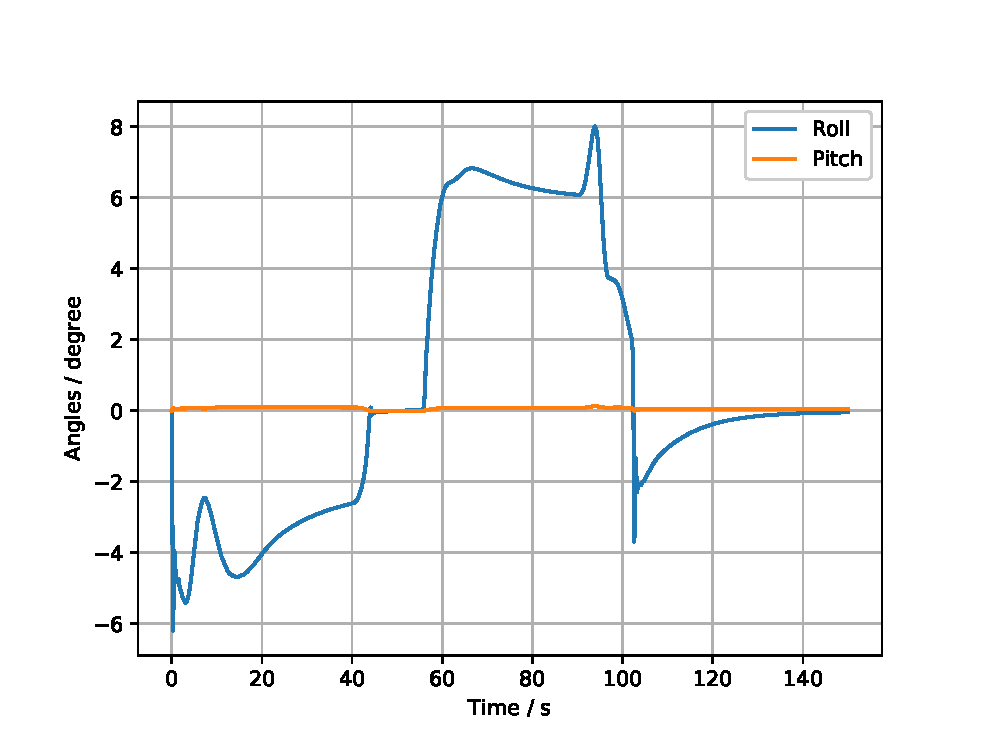
\includegraphics[width = 0.35\linewidth]{documents/figures/angles.eps} \\
%     heading angle & 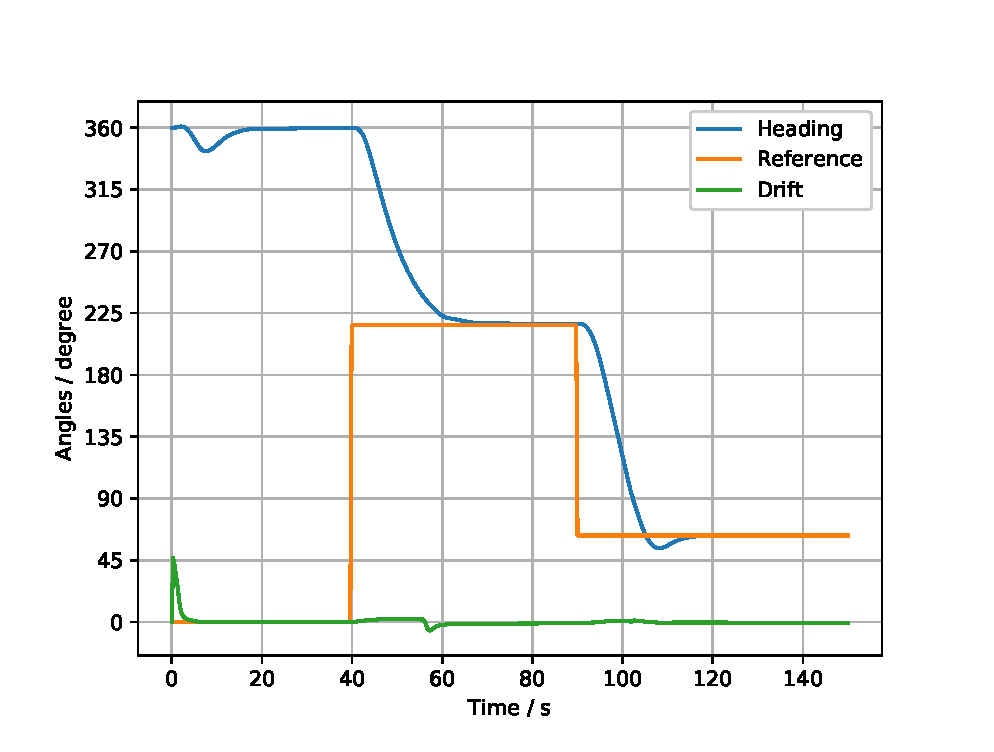
\includegraphics[width = 0.35\linewidth]{documents/figures/heading.eps} & 
%     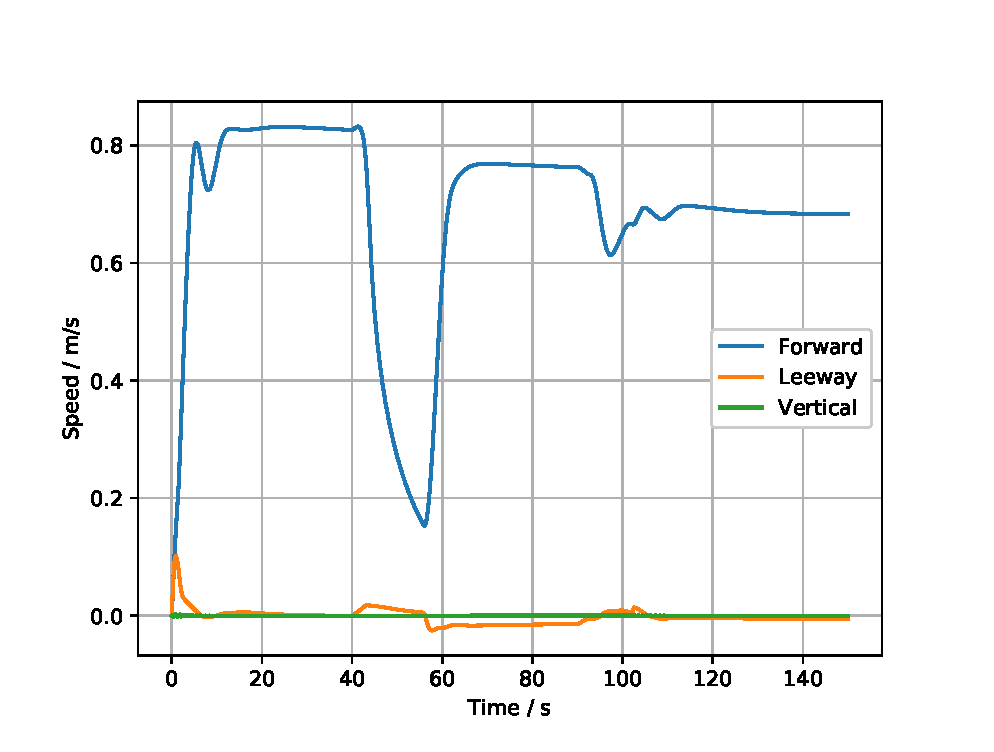
\includegraphics[width = 0.35\linewidth]{documents/figures/speeds.eps}
%     \end{tabular}
%     \caption{Simulator results with example reference headings}
%     \label{tab:plots  }
% \end{table}
% \end{frame}


\section{Control Design}

\begin{frame}{High-level Control Design}

\begin{figure}
    \centering
    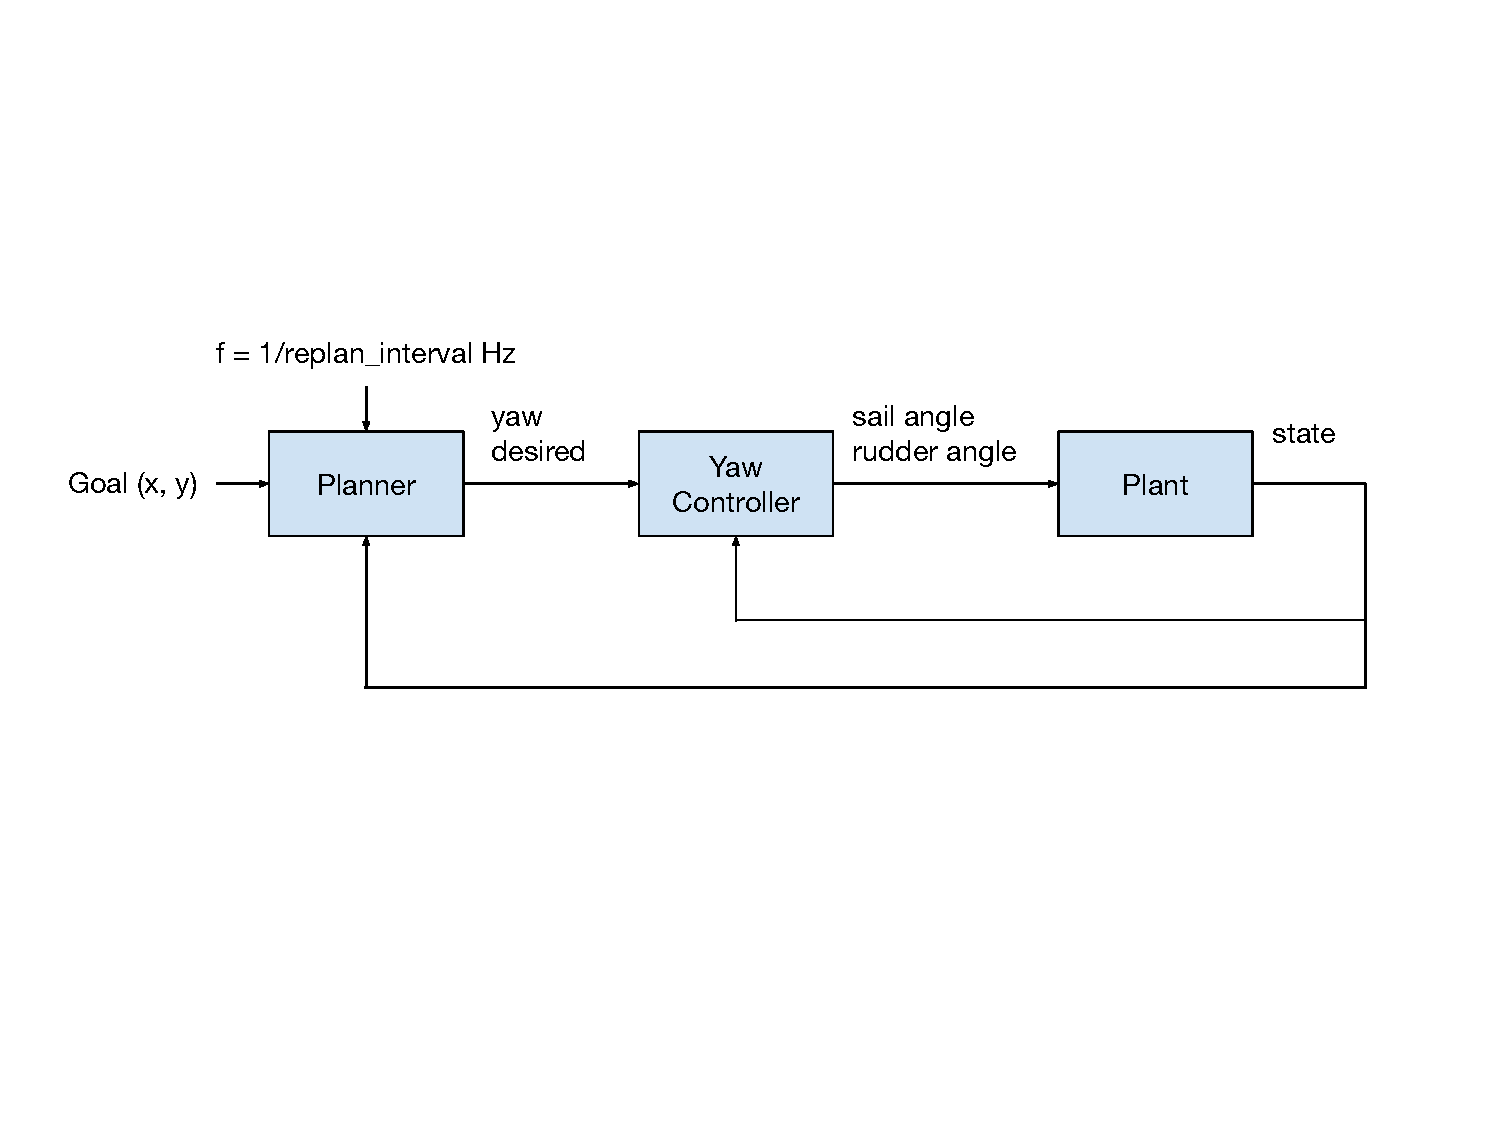
\includegraphics[width=\linewidth,trim={1cm 7cm 2cm 5cm},clip]{documents/final_pres_figs/controller_block_diagram.pdf}
    \caption{Block diagram of planner and controller}
    \label{fig:controller_block_diagram}
\end{figure}
    
A planner generates a reference heading (yaw) for the boat to reach a given \(x, y\) coordinate goal
and boat state.
The planner is run at a low rate since planning, and also the boat itself, is slow.

\hfill\\
The yaw controller generates sail angles and rudder angles to be used as inputs to the boat to
track the reference heading.

\end{frame}

\begin{frame}{Yaw Controller}

The yaw controller is a PID controller from the same paper which developed the simulator and 
model we are using\cite{Buehler2018}.

This controller leverages the fact that there is an optimal angle for the sail based on wind direction to decouple the rudder and sail angle control.

\hfill\\
Apparent wind is the wind relative to the boat (accounting for boat velocity).

\hfill\\
With \(\theta_{aw}\) being the angle of the apparent wind, sail angle is optimally set based on current boat yaw as 
\begin{equation}
    \theta_{\text{sail}} = \frac{\sin(\theta_{aw})}{\cos(\theta_{aw}) + 0.4\cos^2(\theta_{aw})}
\end{equation}
This is clipped based on sailboat limit.
    
\end{frame}

\begin{frame}{Planner}
    
\end{frame}

\begin{frame}{Planner: Boat model}

\end{frame}

\begin{frame}{Planner: Obstacles}

\end{frame}

\section{Experiments and Results}

\section{Conclusion}

\begin{frame}{Future Work and Improvements}
    
\end{frame}

\begin{frame}{Conclusion}
    
\end{frame}

\begin{frame}{Thank You}
    Questions?
\end{frame}


\begin{frame}{References}
    \printbibliography{}
\end{frame}

\end{document}